
\begin{figure}[H] % Use the figure environment
\begin{center}
\resizebox{0.8\textwidth}{!}{ % Scales the figure to fit an A4-sized paper width
\begin{tikzpicture}
    \begin{axis}[
         width=\textwidth, % Set the width to fit the entire page width
        height=0.6\textheight, % Set the height to 60% of the page height
        ybar, 
        symbolic x coords={Direct Query, MV}, % Labels for x-axis
        xtick=data, 
        ylabel={CPU Usage (\%)}, % Y-axis Label (updated to CPU Usage)
        xlabel={Query Execution Type}, % X-axis Label
        nodes near coords, % Shows values above bars
        bar width=35pt, % Adjusted bar width
        enlarge x limits=0.5, % Spacing between bars
        ymin=0, ymax=100, % Y-axis limits
        area legend, % Enables legend area
        legend style={
            at={(0.5,-0.25)}, % Position of the legend (below the chart)
            anchor=north, % Anchors the legend to the north (top) of the point
            yshift=-5pt, % Adds a small gap between xlabel and legend
            font=\small, % Smaller font for legend
        }, 
        bar shift=0pt, % Aligns bars properly
        ymajorgrids=true, % Adds horizontal grid lines
        xmajorgrids=true, % Adds vertical grid lines
        tick style={line width=0.5pt, gray!50},
        grid style={line width=0.2pt,draw=gray!30,dashed}, % Grid line style
        ytick={0, 20, 40, 60, 80, 100}, % Custom Y-axis ticks
        xticklabel style={font=\small}, % Smaller font for x-axis labels
        yticklabel style={font=\small}, % Smaller font for y-axis labels
        axis on top, % Places axis lines on top of the bars
    ]
    \addplot[
        fill=red!30, % First bar fill color (red)
        draw=red, % First bar border color (red)
    ] coordinates {(Direct Query, 62.40)(MV, 51.78)}; % First bar value (Before MV)
   % \addlegendentry{Before MV} % Legend entry for the first bar

    \addplot[
        fill=green!30, % Second bar fill color (green)
        draw=green, % Second bar border color (green)
    ] coordinates {(MV, 51.78)(MV, 51.78)}; % Second bar value (After MV)
    %\addlegendentry{After MV} % Legend entry for the second bar

    \end{axis}
\end{tikzpicture}
}
\caption{Comparison of CPU Usage}
\label{fig:cpu_usage}
\end{center}
\end{figure}